\documentclass[12pt]{article}
\usepackage[a4paper,margin=1.25cm]{geometry}
\usepackage{amsmath,amssymb,mathtools}
\usepackage{graphicx}
\usepackage{booktabs}
\usepackage{tabularx}
\usepackage{tikz}
\usepackage[T1]{fontenc}
\usepackage[utf8]{inputenc}
\usepackage[english]{babel}

\setlength{\parindent}{0pt}
\setlength{\parskip}{0.45em}
\setlength{\abovedisplayskip}{5pt plus 1pt minus 1pt}
\setlength{\belowdisplayskip}{5pt plus 1pt minus 1pt}
\setlength{\abovedisplayshortskip}{3pt plus 1pt minus 1pt}
\setlength{\belowdisplayshortskip}{3pt plus 1pt minus 1pt}

\newcommand{\dd}{\,\mathrm{d}}
\newcommand{\e}{\mathrm{e}}
\newcommand{\In}{I_n}
\newcommand{\Jn}{J_n}

\begin{document}

\begin{center}
{\Large\bfseries A tangent power integral}\\[0.35em]
{\large the perturbation \(1+x^n\) is invisible in the limit}
\end{center}

\[
\boxed{\displaystyle
\lim_{n\to\infty}
\frac{n^2+1}{n}
\int_0^{\pi/4}
\frac{\tan^n x}{1+x^n}\dd x
=\frac12.}
\]

\textbf{Overview.}
Two independent facts do all the work. First, the pure tangent moments
\[
\Jn=\int_0^{\pi/4}\tan^n x\dd x
\]
satisfy an exact two-term recurrence which pins them between
\(\frac1{2(n+1)}\) and \(\frac1{2(n-1)}\); hence \(n\Jn\to\frac12\).
Second, on the interval of integration \(x\le\pi/4<1\), so the
denominator \(1+x^n\) differs from \(1\) by an amount that decays
geometrically, while the integral itself decays only like \(1/n\). A
geometric error against an algebraic main term is negligible, and the
perturbed integral has the same limit as the unperturbed one.

Throughout,
\[
\In=\int_0^{\pi/4}\frac{\tan^n x}{1+x^n}\dd x,
\qquad
\Jn=\int_0^{\pi/4}\tan^n x\dd x,
\qquad n\ge0.
\]

\section*{1. Where the mass sits}

On \([0,\pi/4]\) the integrand \(\tan^n x\) is increasing, with maximum
value \(\tan(\pi/4)=1\) attained at the right endpoint. Every other point
contributes a quantity that is exponentially small in \(n\) relative to
the endpoint: if \(\tan x_0=\theta<1\), then \(\tan^n x_0=\theta^n\).
So the whole integral is produced by a shrinking neighbourhood of
\(x=\pi/4\).

Near that endpoint, with \(t=\frac{\pi}{4}-x\),
\[
\tan\!\left(\frac\pi4-t\right)
=\frac{1-\tan t}{1+\tan t}
=1-2t+O(t^2),
\]
so \(\tan^n x\approx \e^{-2nt}\). The effective width of the peak is
\(t\sim\frac1{2n}\) and the height is \(1\), which already predicts
\[
\Jn\approx\frac1{2n}.
\tag{1}
\]
The next section proves this without any asymptotic analysis.

\begin{center}
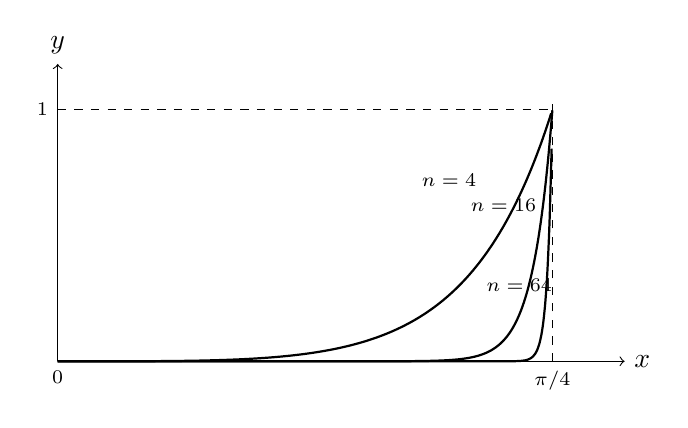
\begin{tikzpicture}[x=8cm,y=3.2cm]
\draw[->] (0,0)--(0.90,0) node[right] {\(x\)};
\draw[->] (0,0)--(0,1.18) node[above] {\(y\)};
\draw[dashed] (0.785398,0)--(0.785398,1.02);
\draw[dashed] (0,1)--(0.785398,1);
\node[below] at (0,0) {\scriptsize \(0\)};
\node[below] at (0.785398,0) {\scriptsize \(\pi/4\)};
\node[left] at (0,1) {\scriptsize \(1\)};
\draw[thick,samples=200,domain=0:0.785398,smooth]
  plot (\x,{pow(tan(\x r),4)});
\draw[thick,samples=220,domain=0:0.785398,smooth]
  plot (\x,{pow(tan(\x r),16)});
\draw[thick,samples=240,domain=0:0.785398,smooth]
  plot (\x,{pow(tan(\x r),64)});
\node[anchor=east] at (0.68,0.72) {\scriptsize \(n=4\)};
\node[anchor=east] at (0.775,0.62) {\scriptsize \(n=16\)};
\node[anchor=east] at (0.80,0.30) {\scriptsize \(n=64\)};
\end{tikzpicture}
\end{center}

\section*{2. The exact recurrence for \(\Jn\)}

The identity \((\tan^{n+1}x)'=(n+1)\tan^n x\,(1+\tan^2x)\) gives, for
\(n\ge0\),
\[
\Jn+J_{n+2}
=\int_0^{\pi/4}\tan^n x\,(1+\tan^2 x)\dd x
=\left[\frac{\tan^{n+1}x}{n+1}\right]_0^{\pi/4}
=\frac1{n+1}.
\tag{2}
\]
This is exact; no estimate has been used yet.

Since \(0\le\tan x\le1\) on \([0,\pi/4]\), the sequence \(\Jn\) is
non-increasing:
\[
J_{n+2}\le \Jn\le J_{n-2},\qquad n\ge2.
\tag{3}
\]
Feeding (3) into (2) in the two possible directions gives a two-sided
bound with no error terms. From \(J_{n+2}\le\Jn\),
\[
\frac1{n+1}=\Jn+J_{n+2}\le 2\Jn,
\]
and from \(\Jn\le J_{n-2}\),
\[
2\Jn\le J_{n-2}+\Jn=\frac1{n-1}.
\]
Hence
\[
\boxed{\displaystyle
\frac1{2(n+1)}\le \Jn\le\frac1{2(n-1)},\qquad n\ge2.}
\tag{4}
\]
In particular
\[
\left|\Jn-\frac1{2n}\right|\le\frac1{2n(n-1)},
\qquad
\lim_{n\to\infty}n\Jn=\frac12,
\tag{5}
\]
which confirms the heuristic (1). Multiplying (4) by
\(\frac{n^2+1}{n}\),
\[
\frac{n^2+1}{2n(n+1)}
\le\frac{n^2+1}{n}\Jn
\le\frac{n^2+1}{2n(n-1)},
\]
and both bounds tend to \(\frac12\), so
\[
\boxed{\displaystyle
\lim_{n\to\infty}\frac{n^2+1}{n}\Jn=\frac12.}
\tag{6}
\]

\section*{3. The perturbation is geometrically small}

Only now does the denominator enter. Since \(0\le x\le\frac\pi4<1\),
\[
0\le\frac{x^n}{1+x^n}\le x^n\le\left(\frac\pi4\right)^n.
\tag{7}
\]
Therefore
\[
\begin{aligned}
0\le \Jn-\In
&=\int_0^{\pi/4}\tan^n x\left(1-\frac1{1+x^n}\right)\dd x\\
&=\int_0^{\pi/4}\tan^n x\,\frac{x^n}{1+x^n}\dd x
\le\left(\frac\pi4\right)^n\Jn.
\end{aligned}
\tag{8}
\]
Multiplying by \(\frac{n^2+1}{n}\) and using the upper bound in (4),
\[
0\le\frac{n^2+1}{n}(\Jn-\In)
\le\left(\frac\pi4\right)^n\frac{n^2+1}{2n(n-1)}
\longrightarrow0,
\tag{9}
\]
because \(\pi/4<1\) and a geometric factor beats the bounded factor
\(\frac{n^2+1}{2n(n-1)}\to\frac12\).

Combining (6) and (9),
\[
\lim_{n\to\infty}\frac{n^2+1}{n}\In
=\lim_{n\to\infty}\frac{n^2+1}{n}\Jn
-\lim_{n\to\infty}\frac{n^2+1}{n}(\Jn-\In)
=\frac12-0,
\]
which is the assertion.

\section*{4. Closed form of the tangent moments}

The recurrence (2) can be unwound. Starting from
\[
J_0=\frac\pi4,
\qquad
J_1=\int_0^{\pi/4}\tan x\dd x=\left[-\log\cos x\right]_0^{\pi/4}
=\frac{\log2}{2},
\]
and writing \(J_{n+2}=\frac1{n+1}-\Jn\), induction gives
\[
J_{2m}=(-1)^m\left(\frac\pi4-\sum_{k=0}^{m-1}\frac{(-1)^k}{2k+1}\right),
\qquad
J_{2m+1}=(-1)^m\left(\frac{\log2}{2}-\sum_{k=0}^{m-1}\frac{(-1)^k}{2k+2}\right).
\tag{10}
\]
So \(\Jn\) is exactly the alternating tail of the Leibniz series for
\(\pi/4\) in the even case, and of the alternating harmonic series for
\(\frac12\log2\) in the odd case. Both classical series have tails of size
\(\frac1{2n}+O(n^{-2})\), which is (5) again, now with the constant
identified in a second way.

\section*{5. What the sandwich looks like}

The table records the two bounds of (4) rescaled, together with the exact
value of the perturbed integral. All three columns approach \(\frac12\);
the last two differ by an amount too small to display already at
\(n=20\), because their gap is controlled by \((\pi/4)^n\).

\begin{center}
\small
\renewcommand{\arraystretch}{1.35}
\begin{tabularx}{0.92\textwidth}{@{}lXXX@{}}
\toprule
\(n\)
& \(\dfrac{n^2+1}{2n(n+1)}\) (lower)
& \(\dfrac{n^2+1}{2n(n-1)}\) (upper)
& gap factor \((\pi/4)^n\) \\
\midrule
\(5\)   & \(0.4333\) & \(0.6500\) & \(3.0\cdot10^{-1}\) \\
\(10\)  & \(0.4591\) & \(0.5611\) & \(9.1\cdot10^{-2}\) \\
\(20\)  & \(0.4774\) & \(0.5276\) & \(8.4\cdot10^{-3}\) \\
\(50\)  & \(0.4906\) & \(0.5104\) & \(6.6\cdot10^{-6}\) \\
\(100\) & \(0.4951\) & \(0.5051\) & \(4.3\cdot10^{-11}\) \\
\bottomrule
\end{tabularx}
\end{center}

\section*{6. The general principle}

Nothing in the argument used the specific shape of \(1+x^n\). The proof
is an instance of the following statement.

\textbf{Proposition.}
Let \(f:[0,a]\to[0,1]\) be continuous with \(f(a)=1\) and \(f<1\) on
\([0,a)\), and let \(a<1\). Let \(\rho_n(x)\) satisfy
\(|1-\rho_n(x)|\le C q^n\) with \(q<1\), uniformly on \([0,a]\). If
\(c_n\int_0^a f^n\to L\) with \(c_n\) growing at most polynomially, then
\[
\lim_{n\to\infty}c_n\int_0^a f(x)^n\rho_n(x)\dd x=L.
\]

\textit{Proof.} The difference is bounded by
\(Cq^n c_n\int_0^a f^n\), and \(c_n\int_0^a f^n\) is bounded while
\(q^n\to0\). \(\square\)

For our problem \(f=\tan\), \(a=\pi/4\), \(\rho_n=(1+x^n)^{-1}\),
\(q=\pi/4\), \(c_n=\frac{n^2+1}{n}\), and \(L=\frac12\). The only
task-specific input is (4), the two-sided bound for \(\Jn\), and that
came from the exact recurrence (2).

Two remarks on the shape of the problem. The factor \(\frac{n^2+1}{n}\)
is a disguised \(n\): its ratio to \(n\) is \(1+n^{-2}\to1\), so it is
present only to make the answer look less like the standard normalisation
\(n\Jn\to\frac12\). And the value \(a=\pi/4\) is doing two separate jobs
at once. It is the point where \(\tan\) reaches \(1\), which is what
makes the integral decay algebraically rather than geometrically, and it
is smaller than \(1\), which is what makes the perturbation decay
geometrically. Had the upper limit been larger than \(1\), the estimate
(7) would fail and the denominator would change the answer.

\end{document}
